\documentclass[aspectratio=169,11pt]{beamer}
\usetheme{Madrid}
\usecolortheme{whale}
\definecolor{uddblue}{HTML}{1F4E79}
\definecolor{uddlight}{HTML}{2E86C1}
\setbeamercolor{structure}{fg=uddblue}
\setbeamercolor{frametitle}{bg=uddblue,fg=white}
\setbeamercolor{title}{bg=uddblue,fg=white}
\setbeamercolor{block title}{bg=uddblue,fg=white}
\setbeamercolor{block body}{bg=uddblue!10}
\setbeamercolor{item}{fg=uddblue}
\usepackage[utf8]{inputenc}
\usepackage[T1]{fontenc}
\usepackage[english]{babel}
\usepackage{amsmath,amssymb}
\usepackage{graphicx}
\usepackage{booktabs}
\usepackage{listings}
\usepackage{tikz}
\usetikzlibrary{shapes,arrows,positioning,calc}
\lstset{language=R,basicstyle=\ttfamily\scriptsize,keywordstyle=\color{uddblue}\bfseries,commentstyle=\color{gray},stringstyle=\color{uddlight},backgroundcolor=\color{uddblue!5},frame=single,rulecolor=\color{uddblue!30},breaklines=true,showstringspaces=false}
\graphicspath{{figuras/}}
\titlegraphic{
\includegraphics[height=1.2cm]{logo_gobierno.png}}
\institute[CICS — UDD]{Doctorado en Ciencias de la Complejidad Social — CICS, UDD}
\date{19 de marzo de 2026}

\title{Sesión 3: Distribuciones de Probabilidad}
\author[A. Agüero]{Amaru Agüero}

\begin{document}

%===============================================
% DIAPOSITIVA 1: Portada
%===============================================
\frame{\titlepage}

%===============================================
% DIAPOSITIVA 2: Agenda
%===============================================
\begin{frame}{Agenda de la sesión}
\tableofcontents[hideallsubsections]
\end{frame}

%===============================================
% SECCIÓN 1: DISTRIBUCIONES DISCRETAS
%===============================================
\section{Distribuciones Discretas}

\begin{frame}{Distribuciones Discretas}
\begin{itemize}
  \item Las distribuciones discretas modelan variables aleatorias que toman un número finito o contable de valores.
  \pause
  \item Características:
  \begin{itemize}
    \item Función de Masa de Probabilidad (PMF): $P(X = x)$
    \item Probabilidades suman 1
    \item Aplicaciones: conteos, eventos sí/no
  \end{itemize}
  \pause
  \item Principales distribuciones:
  \begin{itemize}
    \item Distribución de Bernoulli
    \item Distribución Binomial
    \item Distribución de Poisson
  \end{itemize}
\end{itemize}
\end{frame}

%===============================================
% DIAPOSITIVA 4: Distribución Bernoulli
%===============================================
\begin{frame}{Distribución de Bernoulli}
\begin{block}{Definición}
Experimento con dos resultados posibles: éxito (1) o fracaso (0).
\end{block}

\pause
\begin{columns}[T]
\column{0.5\textwidth}
\textbf{Función de Masa de Probabilidad:}
\[
P(X = x) = p^x(1-p)^{1-x}, \quad x \in \{0,1\}
\]
donde $p$ es la probabilidad de éxito, $0 < p < 1$.

\pause
\textbf{Parámetros:}
\begin{align*}
\text{Media:} \quad &\mu = p \\
\text{Varianza:} \quad &\sigma^2 = p(1-p)
\end{align*}

\column{0.5\textwidth}
\textbf{Ejemplo:}
\begin{itemize}
  \item Lanzar una moneda
  \item Resultado de una pregunta sí/no
  \item Votación sobre una propuesta
\end{itemize}

\pause
Si $p = 0.6$:
\begin{align*}
P(X = 1) &= 0.6 \\
P(X = 0) &= 0.4
\end{align*}
\end{columns}
\end{frame}

%===============================================
% DIAPOSITIVA 5: Distribución Binomial
%===============================================
\begin{frame}{Distribución Binomial}
\small
\begin{block}{Definición}
Suma de $n$ ensayos de Bernoulli independientes, cada uno con probabilidad de éxito $p$.
\end{block}

\pause
\begin{columns}[T]
\column{0.55\textwidth}
\textbf{Función de Masa de Probabilidad:}
\[
P(X = k) = \binom{n}{k}p^k(1-p)^{n-k}
\]
donde $k = 0, 1, \ldots, n$.

\pause
\textbf{Parámetros:}
Media: $\mu = np$, \quad Varianza: $\sigma^2 = np(1-p)$

\column{0.45\textwidth}
\textbf{Aplicaciones:}
\begin{itemize}\setlength{\itemsep}{0pt}
  \item Encuestas: número de personas a favor
  \item Votaciones: cantidad de votos
  \item Control de calidad: defectos en lote
\end{itemize}

\pause
\textbf{Ejemplo numérico:}
Si $n=10$, $p=0.5$:
\[
P(X=5) = \binom{10}{5}(0.5)^5(0.5)^5 \approx 0.246
\]
\end{columns}
\end{frame}

%===============================================
% DIAPOSITIVA 6: Binomial - Visualización
%===============================================
\begin{frame}[fragile]{Distribución Binomial: Ejemplo}
\centering
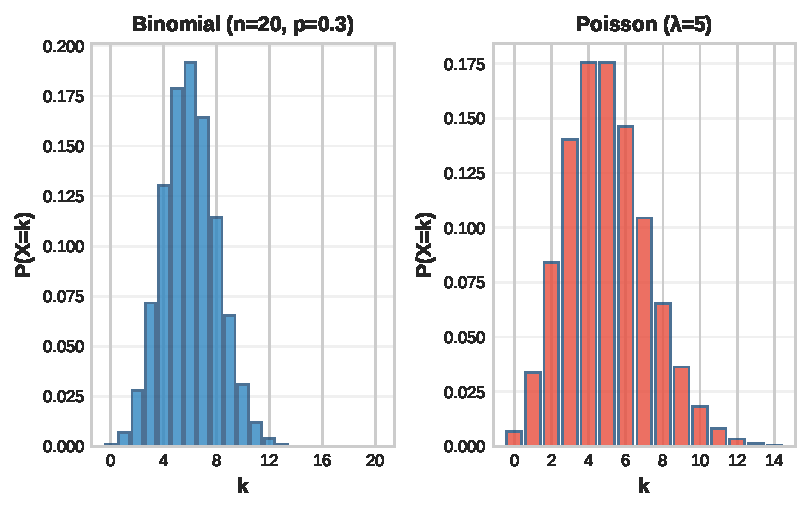
\includegraphics[width=0.7\textwidth,height=0.55\textheight,keepaspectratio]{binomial_poisson.pdf}

\pause
\vspace{0.3cm}
\textbf{Interpretación:} Dado $n=20$ ensayos con $p=0.4$, la probabilidad máxima ocurre alrededor de $k = 8$ éxitos.
\end{frame}

%===============================================
% DIAPOSITIVA 7: Distribución de Poisson
%===============================================
\begin{frame}{Distribución de Poisson}
\small
\begin{block}{Definición}
Modela el número de eventos en un intervalo fijo de tiempo o espacio, con tasa promedio $\lambda$.
\end{block}

\pause
\begin{columns}[T]
\column{0.55\textwidth}
\textbf{Función de Masa de Probabilidad:}
\[
P(X = k) = \frac{e^{-\lambda}\lambda^k}{k!}, \quad k = 0, 1, 2, \ldots
\]
donde $\lambda > 0$ es el parámetro de tasa.

\pause
\textbf{Parámetros:}
Media: $\mu = \lambda$, \quad Varianza: $\sigma^2 = \lambda$

\column{0.45\textwidth}
\textbf{Aplicaciones:}
\begin{itemize}\setlength{\itemsep}{0pt}
  \item Crímenes por zona en un período
  \item Llamadas telefónicas por hora
  \item Accidentes por día
  \item Llegadas a una cola
\end{itemize}

\pause
\textbf{Ejemplo:}
Si $\lambda = 3$ crímenes/semana:
\[
P(X=2) = \frac{e^{-3} \cdot 3^2}{2!} \approx 0.224
\]
\end{columns}
\end{frame}

%===============================================
% DIAPOSITIVA 8: Poisson - Visualización
%===============================================
\begin{frame}[fragile]{Distribución de Poisson: Ejemplo}
\centering
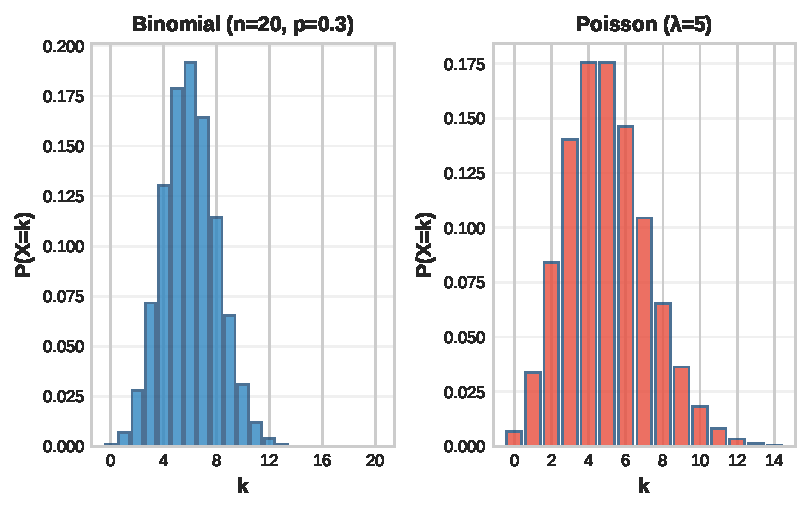
\includegraphics[width=0.7\textwidth,height=0.55\textheight,keepaspectratio]{binomial_poisson.pdf}

\pause
\vspace{0.3cm}
\textbf{Interpretación:} Para $\lambda = 4$, la probabilidad se concentra alrededor de 4 eventos, con cola decreciente.

\pause
\textbf{Nota:} La distribución de Poisson es el límite de la Binomial cuando $n \to \infty$, $p \to 0$ y $np = \lambda$.
\end{frame}

%===============================================
% SECCIÓN 2: DISTRIBUCIÓN NORMAL
%===============================================
\section{Distribución Normal}

%===============================================
% DIAPOSITIVA 9: Distribución Normal - Introducción
%===============================================
\begin{frame}{Distribución Normal}
\begin{block}{Definición}
La distribución normal (o gaussiana) es la más importante en estadística. Describe muchos fenómenos naturales.
\end{block}

\pause
\begin{columns}[T]
\column{0.55\textwidth}
\textbf{Función de Densidad de Probabilidad (PDF):}
\[
f(x) = \frac{1}{\sigma\sqrt{2\pi}} \exp\left(-\frac{(x-\mu)^2}{2\sigma^2}\right)
\]

\textbf{Parámetros:}
\begin{itemize}
  \item $\mu$ = media (desplaza la curva)
  \item $\sigma$ = desviación estándar (controla amplitud)
\end{itemize}

\pause
\textbf{Notación:} $X \sim N(\mu, \sigma^2)$

\column{0.45\textwidth}
\textbf{Propiedades:}
\begin{itemize}
  \item Forma de campana simétrica
  \item Unimodal (un pico)
  \item Media = Mediana = Moda
  \item Asintótica en los extremos
\end{itemize}

\pause
\textbf{Aplicaciones:}
\begin{itemize}
  \item Altura, peso
  \item Errores de medición
  \item Calificaciones
\end{itemize}
\end{columns}
\end{frame}

%===============================================
% DIAPOSITIVA 10: Distribución Normal - Visualización
%===============================================
\begin{frame}{Distribución Normal: Forma y Propiedades}
\centering
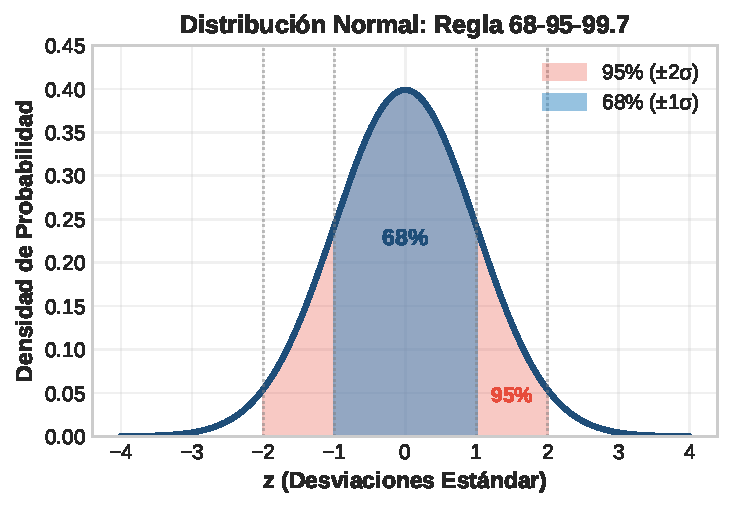
\includegraphics[width=0.8\textwidth,height=0.55\textheight,keepaspectratio]{distribucion_normal.pdf}

\pause
\vspace{0.2cm}
\textbf{Cambios en $\mu$ y $\sigma$ afectan la posición y amplitud de la curva.}
\end{frame}

%===============================================
% DIAPOSITIVA 11: Regla Empírica
%===============================================
\begin{frame}{Regla Empírica (68-95-99.7)}
Para una distribución normal $N(\mu, \sigma^2)$:

\vspace{0.3cm}
\begin{columns}[T]
\column{0.55\textwidth}
\begin{itemize}
  \item \textbf{68\%} de los datos caen en $[\mu - \sigma, \mu + \sigma]$
  \item \textbf{95\%} de los datos caen en $[\mu - 2\sigma, \mu + 2\sigma]$
  \item \textbf{99.7\%} de los datos caen en $[\mu - 3\sigma, \mu + 3\sigma]$
\end{itemize}

\vspace{0.3cm}
\textbf{Implicaciones:}
\begin{itemize}
  \item Observaciones $> 3\sigma$ de la media son muy raras
  \item Esta regla es aproximada pero muy útil en la práctica
\end{itemize}

\column{0.45\textwidth}
\centering
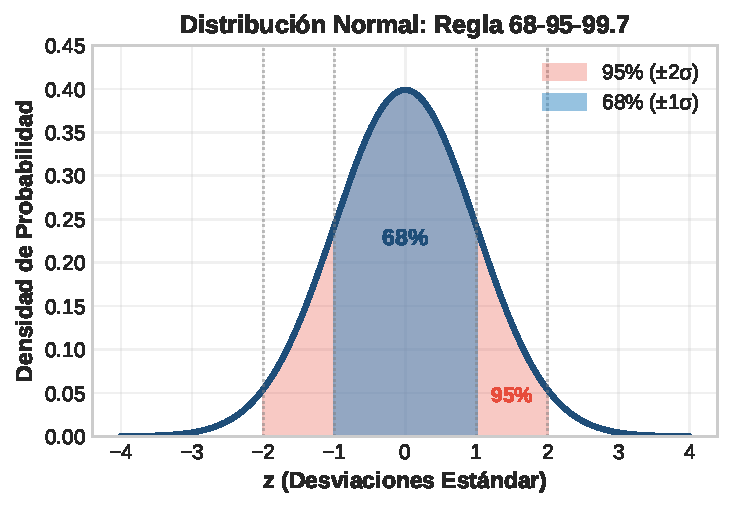
\includegraphics[width=\linewidth,height=0.6\textheight,keepaspectratio]{distribucion_normal.pdf}
\end{columns}
\end{frame}

%===============================================
% DIAPOSITIVA 12: Distribución Normal Estándar
%===============================================
\begin{frame}{Distribución Normal Estándar y Estandarización}
\small
\begin{block}{Estandarización (Z-score)}
Convertir $X \sim N(\mu, \sigma^2)$ a la estándar $N(0,1)$: \quad $Z = \dfrac{X - \mu}{\sigma}$
\end{block}

\pause
\begin{columns}[T]
\column{0.55\textwidth}
\textbf{Ventajas:}
\begin{itemize}\setlength{\itemsep}{0pt}
  \item Una sola tabla de referencias
  \item Comparabilidad entre variables diferentes
  \item $P(X \leq x) = P(Z \leq z)$
\end{itemize}

\pause
\textbf{Ejemplo:}
Si $X \sim N(100, 15^2)$ y queremos $P(X \leq 115)$:
$Z = \frac{115 - 100}{15} = 1$, \quad luego $P(X \leq 115) = P(Z \leq 1) \approx 0.841$

\column{0.45\textwidth}
\textbf{En R:}
\begin{lstlisting}
# Probabilidad acumulada
pnorm(1)  # ~0.841

# Cuantil (inversa)
qnorm(0.841)  # ~1
\end{lstlisting}

\pause
\textbf{Interpretación:} El 84.1\% de los datos está bajo $x = 115$.
\end{columns}
\end{frame}

%===============================================
% DIAPOSITIVA 13: Funciones R para Normal
%===============================================
\begin{frame}[fragile]{Funciones R: Distribución Normal}
\begin{columns}[T]
\column{0.5\textwidth}
\textbf{pnorm(): Función acumulada (CDF)}
\begin{lstlisting}
# P(X ≤ 1) para N(0,1)
pnorm(1)

# P(X ≤ 115) para N(100,15)
pnorm(115, mean=100, sd=15)

# Prob. cola superior
1 - pnorm(1)
\end{lstlisting}

\pause
\column{0.5\textwidth}
\textbf{qnorm(): Cuantiles (inversa CDF)}
\begin{lstlisting}
# Encontrar z tal que P(Z ≤ z) = 0.975
qnorm(0.975)

# Percentil 95 de N(100, 15²)
qnorm(0.95, mean=100, sd=15)

# Intervalo de confianza 95%
qnorm(c(0.025, 0.975))
\end{lstlisting}
\end{columns}

\pause
\vspace{0.3cm}
\begin{block}{Importante}
\texttt{pnorm()} da probabilidades (área bajo la curva). \texttt{qnorm()} da valores de la variable.
\end{block}
\end{frame}

%===============================================
% SECCIÓN 3: TEOREMA DEL LÍMITE CENTRAL
%===============================================
\section{Teorema del Límite Central}

%===============================================
% DIAPOSITIVA 14: TLC - Enunciado
%===============================================
\begin{frame}{Teorema del Límite Central (TLC)}
\small
\begin{block}{Enunciado}
Si $X_1, X_2, \ldots, X_n$ son v.a.\ iid con media $\mu$ y varianza $\sigma^2$ finitas, entonces la media muestral
$\overline{X}_n = \frac{1}{n}\sum_{i=1}^{n} X_i$
converge a una distribución normal con media $\mu$ y varianza $\sigma^2/n$ cuando $n \to \infty$.
\end{block}

\pause
\textbf{En símbolos:}
\[
\overline{X}_n \xrightarrow{d} N\left(\mu, \frac{\sigma^2}{n}\right)
\]

\pause
\textbf{Implicación clave:} \textit{La distribución de la media es aproximadamente normal, incluso si la población original no lo es.}
\end{frame}

%===============================================
% DIAPOSITIVA 15: TLC - Intuición
%===============================================
\begin{frame}{Teorema del Límite Central: Intuición}
\begin{columns}[T]
\column{0.6\textwidth}
\textbf{¿Por qué es tan importante?}

\pause
\begin{itemize}
  \item La media de una muestra es más estable que observaciones individuales
  \item A mayor tamaño de muestra $n$, más normal es $\overline{X}_n$
  \item La varianza de $\overline{X}_n$ es $\sigma^2/n$ (disminuye con $n$)
\end{itemize}

\pause
\vspace{0.3cm}
\textbf{Consecuencias para la Inferencia:}
\begin{itemize}
  \item Justifica el uso de la distribución normal
  \item Base para intervalos de confianza
  \item Fundamental en pruebas de hipótesis
\end{itemize}

\column{0.4\textwidth}
\centering
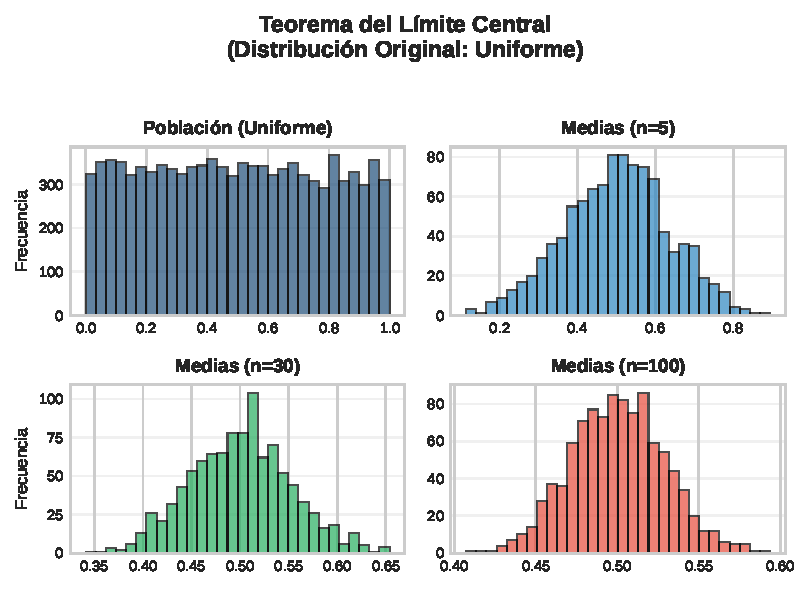
\includegraphics[width=\textwidth,height=0.6\textheight,keepaspectratio]{tlc_simulacion.pdf}

\pause
\footnotesize
\textit{A medida que $n$ aumenta, la distribución de $\overline{X}_n$ se vuelve más normal.}
\end{column}
\end{columns}
\end{frame}

%===============================================
% DIAPOSITIVA 16: TLC - Ejemplo Simulación
%===============================================
\begin{frame}[fragile]{Teorema del Límite Central: Simulación en R}
\begin{lstlisting}[basicstyle=\ttfamily\tiny]
# Simular muestras de distribución no-normal
set.seed(123)
n_muestras <- 10000
n <- 30

medias <- replicate(n_muestras, {
  muestra <- runif(n, min=0, max=10)  # Uniforme
  mean(muestra)
})

# Visualizar
hist(medias, breaks=50, main="Distribución de medias",
     xlab="Media muestral", probability=TRUE)

# Superponer normal teórica
x <- seq(4, 6, by=0.01)
lines(x, dnorm(x, mean=5, sd=sqrt(100/12/n)),
      col="red", lwd=2)
\end{lstlisting}

\vspace{0.15cm}
\textbf{Resultado:} Distribución uniforme → Medias distribuidas normalmente (Teorema del Límite Central confirmado).
\end{frame}

%===============================================
% SECCIÓN 4: DISTRIBUCIONES DERIVADAS
%===============================================
\section{Distribuciones Derivadas}

%===============================================
% DIAPOSITIVA 17: Distribuciones Derivadas - Introducción
%===============================================
\begin{frame}{Distribuciones Derivadas de la Normal}
Cuando trabajamos con estadísticos muestrales (media, varianza), aparecen distribuciones especiales:

\pause
\vspace{0.3cm}
\begin{itemize}
  \item \textbf{Distribución $t$ de Student:} Cuando estimamos $\sigma$ con $s$
  \pause
  \item \textbf{Distribución $\chi^2$ (chi-cuadrado):} Suma de normales al cuadrado
  \pause
  \item \textbf{Distribución $F$ de Fisher:} Razón de varianzas
\end{itemize}

\pause
\vspace{0.3cm}
\begin{block}{Relación con la Normal}
Todas estas distribuciones se derivan de variables normales estándar y son fundamentales para la inferencia estadística.
\end{block}
\end{frame}

%===============================================
% DIAPOSITIVA 18: Distribución t de Student
%===============================================
\begin{frame}{Distribución $t$ de Student}
\small
\begin{block}{Definición}
Si $Z \sim N(0,1)$ y $V \sim \chi^2_{\nu}$ independientes: $T = \frac{Z}{\sqrt{V/\nu}} \sim t_{\nu}$, donde $\nu$ = grados de libertad.
\end{block}

\pause
\begin{columns}[T]
\column{0.5\textwidth}
\textbf{Características:}
\begin{itemize}\setlength{\itemsep}{0pt}
  \item Simétrica alrededor de 0
  \item Colas más pesadas que la normal
  \item Parámetro: $\nu$ (grados de libertad)
  \item $\nu \to \infty \Rightarrow t_\nu \to N(0,1)$
\end{itemize}

\pause
\textbf{Aplicación:}
\begin{itemize}\setlength{\itemsep}{0pt}
  \item IC para $\mu$ con $\sigma$ desconocida
  \item Pruebas $t$ de Student
  \item Muestras pequeñas
\end{itemize}

\column{0.5\textwidth}
\textbf{Ejemplo:} $\nu = 5, 10, 30$ g.l.
\vspace{0.1cm}
\centering
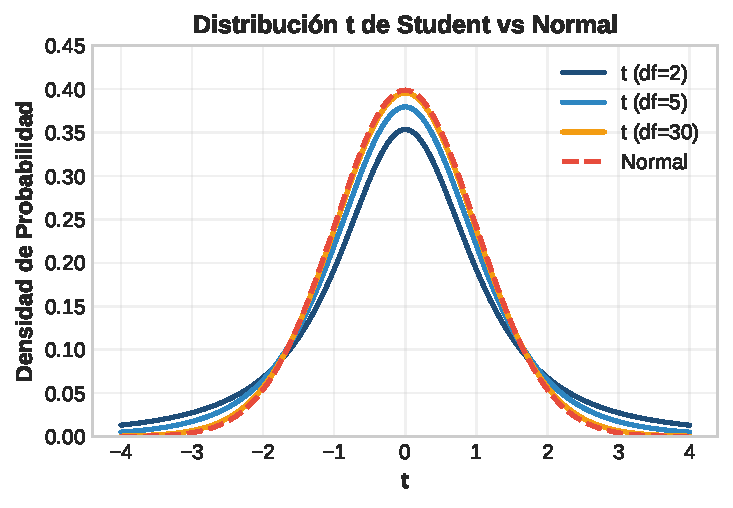
\includegraphics[width=0.85\textwidth]{distribuciones_t.pdf}

\pause
\footnotesize
La $t$ con pocos g.l.\ tiene colas más pesadas.
\end{columns}
\end{frame}

%===============================================
% DIAPOSITIVA 19: Distribución Chi-cuadrado
%===============================================
\begin{frame}{Distribución $\chi^2$ (Chi-cuadrado)}
\begin{block}{Definición}
Si $Z_1, Z_2, \ldots, Z_k$ son normales estándar independientes, entonces
\[
\chi^2_k = \sum_{i=1}^{k} Z_i^2 \sim \chi^2_k
\]
\end{block}

\pause
\begin{columns}[T]
\column{0.5\textwidth}
\textbf{Características:}
\begin{itemize}
  \item Solo toma valores positivos
  \item Asimétrica a la derecha
  \item Parámetro: $k$ (grados de libertad)
  \item Media: $k$, Varianza: $2k$
\end{itemize}

\pause
\textbf{Aplicación:}
\begin{itemize}
  \item Pruebas de bondad de ajuste
  \item Pruebas de independencia
  \item Construcción de intervalos para varianza
\end{itemize}

\column{0.5\textwidth}
\textbf{Comportamiento con distintos $k$:}

\vspace{0.3cm}

\begin{tikzpicture}[scale=0.9]
  \draw[uddblue, thick] plot[smooth, domain=0:10, samples=100]
    (\x, {0.5*(\x/4)^2*exp(-\x/2)/2});
  \draw[uddblue] (0,0) -- (10,0);
  \draw[uddblue] (0,-0.05) -- (0,0.05);
  \node[below, uddblue, font=\tiny] at (2.5,0) {$k=3$};
\end{tikzpicture}

\vspace{0.2cm}
A mayor $k$, la distribución se vuelve más simétrica (acercándose a la normal).
\end{column}
\end{columns}
\end{frame}

%===============================================
% DIAPOSITIVA 20: Distribución F de Fisher
%===============================================
\begin{frame}{Distribución $F$ de Fisher}
\small
\begin{block}{Definición}
Si $U \sim \chi^2_{\nu_1}$ y $V \sim \chi^2_{\nu_2}$ independientes: $F = \frac{U/\nu_1}{V/\nu_2} \sim F_{\nu_1, \nu_2}$
\end{block}

\pause
\begin{columns}[T]
\column{0.5\textwidth}
\textbf{Características:}
\begin{itemize}\setlength{\itemsep}{0pt}
  \item Solo valores positivos
  \item Asimétrica a la derecha
  \item Parámetros: $\nu_1$ (num.), $\nu_2$ (den.)
  \item Razón de dos varianzas muestrales
\end{itemize}

\pause
\textbf{Aplicación:}
\begin{itemize}\setlength{\itemsep}{0pt}
  \item Pruebas $F$ (ANOVA)
  \item Comparación de varianzas
  \item Regresión lineal
\end{itemize}

\column{0.5\textwidth}
\textbf{Relación entre distribuciones:}

\vspace{0.1cm}
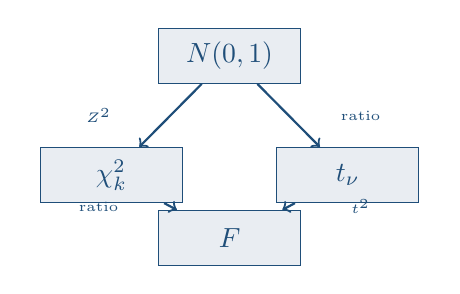
\begin{tikzpicture}[node distance=1.2cm, minimum width=1.8cm, minimum height=0.7cm]
  \node[draw, uddblue, fill=uddblue!10] (normal) {$N(0,1)$};
  \node[draw, uddblue, fill=uddblue!10, below=0.8cm of normal, xshift=-1.5cm] (chi2) {$\chi^2_k$};
  \node[draw, uddblue, fill=uddblue!10, below=0.8cm of normal, xshift=1.5cm] (t) {$t_\nu$};
  \node[draw, uddblue, fill=uddblue!10, below=1.6cm of normal] (f) {$F$};

  \draw[->, uddblue, thick] (normal) -- (chi2) node[midway, left, font=\tiny] {$Z^2$};
  \draw[->, uddblue, thick] (normal) -- (t) node[midway, right, font=\tiny] {ratio};
  \draw[->, uddblue, thick] (chi2) -- (f) node[midway, left, font=\tiny] {ratio};
  \draw[->, uddblue, thick] (t) -- (f) node[midway, right, font=\tiny] {$t^2$};
\end{tikzpicture}
\end{column}
\end{columns}
\end{frame}

%===============================================
% SECCIÓN 5: FUNCIONES EN R
%===============================================
\section{Funciones en R}

%===============================================
% DIAPOSITIVA 21: Generación de variables aleatorias
%===============================================
\begin{frame}[fragile]{Generación de Variables Aleatorias en R}
\textbf{Patrón general:} \texttt{r*} (random), \texttt{d*} (density), \texttt{p*} (probability), \texttt{q*} (quantile)

\pause
\vspace{0.2cm}
\begin{columns}[T]
\column{0.5\textwidth}
\textbf{Distribuciones Discretas}
\begin{lstlisting}
# Bernoulli (rbinom con n=1)
rbinom(n=100, size=1, prob=0.6)

# Binomial
rbinom(n=50, size=20, prob=0.4)

# Poisson
rpois(n=100, lambda=3)
\end{lstlisting}

\column{0.5\textwidth}
\textbf{Distribuciones Continuas}
\begin{lstlisting}
# Normal
rnorm(n=100, mean=0, sd=1)

# t de Student
rt(n=50, df=10)

# Chi-cuadrado
rchisq(n=100, df=5)

# F de Fisher
rf(n=100, df1=5, df2=20)
\end{lstlisting}
\end{columns}

\pause
\vspace{0.3cm}
\begin{block}{Nota}
La función \texttt{set.seed()} fija la semilla para reproducibilidad.
\end{block}
\end{frame}

%===============================================
% DIAPOSITIVA 22: Probabilidades y Cuantiles
%===============================================
\begin{frame}[fragile]{Probabilidades y Cuantiles en R}
\begin{columns}[T]
\column{0.5\textwidth}
\textbf{Función \texttt{p*()}: CDF (Acumulada)}
\begin{lstlisting}
# P(X ≤ 1) para N(0,1)
pnorm(1)

# P(X ≤ 10) para Poisson(5)
ppois(10, lambda=5)

# P(X ≤ 2.5) para t con 10 gl
pt(2.5, df=10)

# Cola superior
1 - pnorm(1)
\end{lstlisting}

\pause
\column{0.5\textwidth}
\textbf{Función \texttt{q*()}: Cuantiles (CDF inversa)}
\begin{lstlisting}
# Hallar q tal que P(Z ≤ q) = 0.95
qnorm(0.95)

# Percentil 90 de N(100, 225)
qnorm(0.90, mean=100, sd=15)

# Intervalo de confianza 95%
qnorm(c(0.025, 0.975))

# Cuartiles de una t
qt(c(0.25, 0.5, 0.75), df=15)
\end{lstlisting}
\end{column}
\end{columns}

\pause
\vspace{0.2cm}
\begin{block}{Regla Mnemotécnica}
\texttt{p} = Prob. acumulada; \texttt{q} = Quantile (inversa); \texttt{r} = Random; \texttt{d} = Density/Probability
\end{block}
\end{frame}

%===============================================
% DIAPOSITIVA 23: Visualización de Distribuciones
%===============================================
\begin{frame}[fragile]{Visualización de Distribuciones}
\begin{lstlisting}[basicstyle=\ttfamily\scriptsize]
# Histograma con curva teórica
set.seed(42)
datos <- rnorm(10000, mean=100, sd=15)
hist(datos, breaks=50, probability=TRUE,
     main="Normal(100, 225)", xlab="Valores")

# Superponer densidad teórica
x <- seq(50, 150, by=1)
lines(x, dnorm(x, mean=100, sd=15), col="red", lwd=2)

# Q-Q plot para verificar normalidad
qqnorm(datos)
qqline(datos, col="red")
\end{lstlisting}

\pause
\small
\textbf{Funciones útiles:}
\begin{itemize}\setlength{\itemsep}{0pt}
  \item \texttt{hist()} para histogramas; \texttt{plot()} y \texttt{lines()} para curvas
  \item \texttt{qqnorm()} para Q-Q plots (evaluar normalidad); \texttt{curve()} para funciones
\end{itemize}
\end{frame}

%===============================================
% SECCIÓN 6: EJERCICIO PRÁCTICO
%===============================================
\section{Ejercicio Práctico}

%===============================================
% DIAPOSITIVA 24: Ejercicio Práctico
%===============================================
\begin{frame}{Ejercicio Práctico: Análisis de Calificaciones}
\small
\begin{block}{Escenario}
Calificaciones $\sim N(\mu = 70, \sigma = 10)$.
\end{block}

\pause
\textbf{Preguntas:}
\begin{enumerate}\setlength{\itemsep}{2pt}
  \item ¿Probabilidad de calificación mayor a 85?
  \pause
  \quad $P(X > 85) = P\!\left(Z > \frac{85-70}{10}\right) = P(Z > 1.5) = 1 - \Phi(1.5)$

  \pause
  \item ¿Percentil 90 de las calificaciones?
  \pause
  \quad $x_{90} = \mu + z_{90} \cdot \sigma = 70 + 1.28 \times 10 = 82.8$

  \pause
  \item Si $n=25$, ¿distribución de $\overline{X}$?
  \pause
  \quad $\overline{X} \sim N(70,\; 10^2/25) = N(70,\; 4) \implies \text{sd}(\overline{X}) = 2$
\end{enumerate}
\end{frame}

%===============================================
% DIAPOSITIVA 25: Ejercicio en R
%===============================================
\begin{frame}[fragile]{Solución en R}
\begin{lstlisting}[basicstyle=\ttfamily\tiny]
# Parámetros
mu <- 70; sigma <- 10

# 1. P(X > 85)
p_mayor_85 <- 1 - pnorm(85, mean=mu, sd=sigma)
print(p_mayor_85)  # 0.0668

# 2. Percentil 90
percentil_90 <- qnorm(0.90, mean=mu, sd=sigma)
print(percentil_90)  # 82.82

# 3. Desv. est. de media muestral (n=25)
n <- 25
se_media <- sigma / sqrt(n)
print(se_media)  # 2

# Simular y verificar
set.seed(123)
medias <- replicate(10000, mean(rnorm(n, mean=mu, sd=sigma)))
sd(medias)  # ~2
\end{lstlisting}

\pause
\small
\textbf{Interpretación:} El 6.68\% de estudiantes obtiene más de 85 puntos.
\end{frame}

%===============================================
% DIAPOSITIVA 26: Resumen
%===============================================
\begin{frame}{Resumen de la Sesión}
\begin{enumerate}
  \item \textbf{Distribuciones Discretas}: Bernoulli, Binomial, Poisson modelan conteos y eventos binarios.
  \pause
  \item \textbf{Distribución Normal}: La más importante; caracterizada por $\mu$ y $\sigma$.
  \pause
  \item \textbf{Teorema del Límite Central}: La media muestral es aproximadamente normal, fundamental para inferencia.
  \pause
  \item \textbf{Distribuciones Derivadas}: $t$, $\chi^2$, $F$ son estadísticos de muestras normales.
  \pause
  \item \textbf{R}: Funciones \texttt{r*}, \texttt{d*}, \texttt{p*}, \texttt{q*} para generar y analizar distribuciones.
\end{enumerate}

\pause
\vspace{0.4cm}
\begin{block}{Siguiente sesión}
Estimación puntual e intervalos de confianza usando estas distribuciones.
\end{block}
\end{frame}

%===============================================
% DIAPOSITIVA 27: Bibliografía y Recursos
%===============================================
\begin{frame}{Recursos Adicionales}
\begin{itemize}
  \item \textbf{R packages:}
  \begin{itemize}
    \item Base R: funciones de distribuciones
    \item \texttt{ggplot2}: visualización avanzada
    \item \texttt{tidyverse}: manipulación de datos
  \end{itemize}
  \pause
  \item \textbf{Referencias:}
  \begin{itemize}
    \item Wasserman, L. (2004). \textit{All of Statistics}. Springer.
    \item Wickham, H., \& Grolemund, G. (2016). \textit{R for Data Science}. O'Reilly.
  \end{itemize}
  \pause
  \item \textbf{En línea:}
  \begin{itemize}
    \item CRAN Task Views
    \item RStudio Cheatsheets
  \end{itemize}
\end{itemize}

\pause
\vspace{0.4cm}
\centering
\Large \textbf{¿Preguntas?}
\end{frame}

\end{document}
